\documentclass[aspectratio=169]{beamer}
\usepackage[utf8]{inputenc}
\usepackage[super]{nth}
\usepackage{censor}
\usepackage{skull}
\usepackage{adjustbox}
\usepackage[binary-units=true, per-mode=symbol]{siunitx}
\usepackage{hyperref}
\usetheme{cern}

% Presentation on CTA at CHEP 2019
% https://indico.cern.ch/event/773049/contributions/3474415/
% 7 Nov 2019, 11:45
% 15m
% Riverbank R8 (Adelaide Convention Centre)

\author{Eric~Cano\thanks{CERN, Geneva}
   \and Vlad\'imir~Bahyl\footnotemark[1]
   \and C\'edric~Caffy\footnotemark[1]
   \and Germ\'an~Cancio\footnotemark[1]
   \and Michael~Davis\footnotemark[1]
   \and Viktor~Kotlyar\thanks{Institute for High Energy Physics, Protvino, Russia}
   \and Julien~Leduc\footnotemark[1]
   \and Giuseppe~Lo~Presti\footnotemark[1]
   \and Tao~Lin\thanks{Institute of High Energy Physics, Chinese Academy of Sciences}
   \and Steven~Murray\footnotemark[1]
}

% The optional `\title` command defines the title and is displayed in the slide produced by the `\titlepage` command.
\title[CTA: production, migration and new features]{CERN Tape Archive: production status, migration from CASTOR and new features}

% The optional `\subtitle` command will add a smaller title below the main one, and will not be displayed in any of the slides' footer.
% \subtitle{}

% The optional `\date` command will display a custom free text date on the all of the slides' footer. If omitted today's date will be used.
\date{CHEP 2019, 7 Nov 2019}

\setcounter{tocdepth}{1}

\begin{document}

\frontcover

% The optional `\titlepage` command will create a slide with the presentation's title, subtitle and author.
\frame{\titlepage}

% The optional `\tableofcontents` command will automatically create a table of contents based pm the sections.
\frame{\tableofcontents}

\section{What is CTA?}
\subsection{What is CTA?}
\begin{frame}{What is CTA?}
\adjustbox{minipage=1.11\textwidth, scale=0.9}{
  \begin{itemize}
    \item The CERN Tape Archive (CTA) is a tape backend for EOS
    \begin{itemize}
      \item EOS is the CERN developed disk system for physics data
    \end{itemize}      
    \item A central CTA is the tape backend for several EOSCTA instances
    \item EOS:
    \begin{itemize}
      \item provides the user interface (XRootd)
      \item holds the directory structure, files metadata
      \item manages disk (HDD or SSD) buffers
      \item handles garbage collection
    \end{itemize}
    \item CTA:
    \begin{itemize}
      \item manages transparently file residence on tape
      \item transfers tape files to/from disk cache on request from EOS
    \end{itemize}
  \end{itemize}
}
\end{frame}

\section{CTA service, integration with EOS and FTS}
\subsection{Current deployment model}
\begin{frame}
	\begin{columns}
		\begin{column}{0.45\textwidth}
			\begin{center}
			  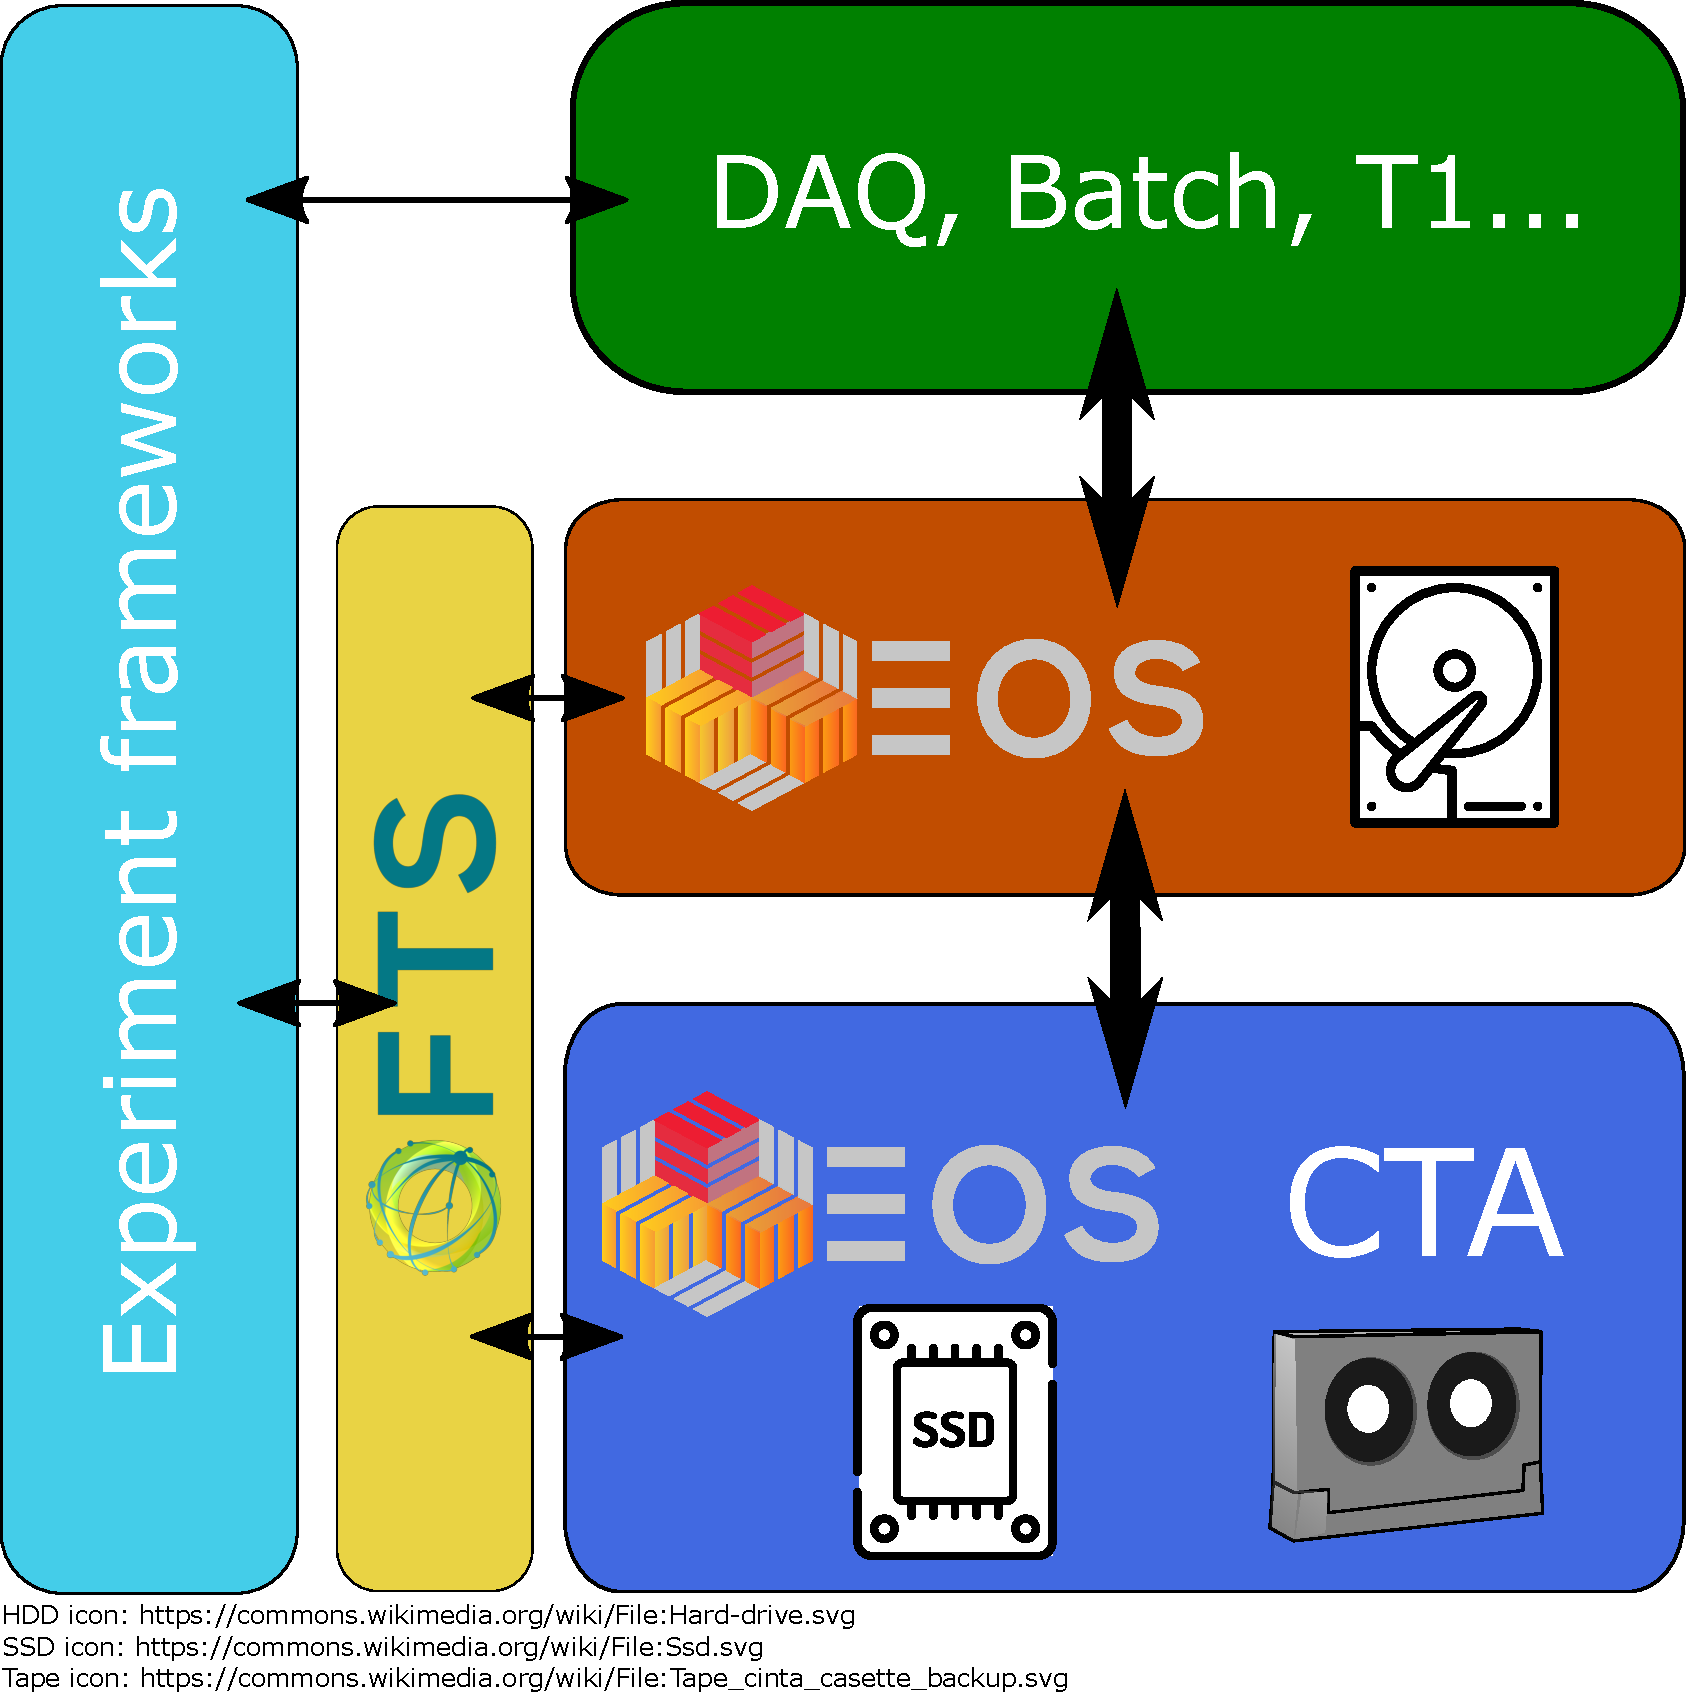
\includegraphics[keepaspectratio, height=1\textheight, width=1\textwidth]{../images/CTA_Deployment_model.pdf}
			\end{center}
		\end{column}
		\begin{column}{0.55\textwidth}
			\adjustbox{minipage=1.30\textwidth, scale=0.8}{{\Huge{}\textcolor{cern}{Current deployment model (I)}}
				\begin{itemize}
				  \item Analysis/DAQ goes through the disk based EOS instance
				  \item EOSCTA instances are dedicated to tape archive
				  \item One EOSCTA instance per experiment, with dedicated namespace and storage space
				  \item CTA is a shared tape service providing tape storage to all EOSCTA instances
				  \item The File Transfer Service (FTS) can manage stage-in and transfers between EOS and EOSCTA
				\end{itemize}
			}
		\end{column}
	\end{columns}
\end{frame}

\begin{frame}{Current deployment model (II)}
% ITTF: https://indico.cern.ch/event/843592/
Plans for CERN T0 deployment
\begin{itemize}
  \item Equipment in procurement
  \item Design validated in smaller scale pre-production
  \item 30 disk servers with $\approx$\SI{1}{\peta\byte} of SSD for buffering
  \item Tape servers transferred from CASTOR 
  \begin{itemize}
    \item Upgrade cycle coming soon
  \end{itemize} 
\end{itemize}
\end{frame}

\subsection{Integration with EOS and FTS}
\begin{frame}{Integration with EOS and FTS}
  \adjustbox{minipage=1.11\textwidth, scale=0.9}{
    \vspace{10pt}
	  \begin{itemize}
	    \item All protocols and disk storage functionality available via EOS
	    \item EOS has been extended to support tape related operations
	    \begin{itemize}
	      \item Lifecycle management
	      \item Stage in
	      \item Cache/buffer management
	      \item Garbage collector
	    \end{itemize}
	    \item More details in \textcolor{cern}{\href{https://indico.cern.ch/event/773049/contributions/3474409/}{``EOS architectural evolution and strategic development directions''}}
	    \item FTS support added for stage in in EOSCTA, transfer to EOS, eviction from buffer
	    \item See also \textcolor{cern}{\href{https://indico.cern.ch/event/773049/contributions/3474419/}{``FTS improvements for LHC Run-3 and beyond''}}
	  \end{itemize}
  }
\end{frame}

\subsection{Integration with experiments work flows and results}
\begin{frame}{Integration with experiments: ATLAS}
\begin{columns}
	\begin{column}{0.40\textwidth}
		\begin{center}
		  \includegraphics[keepaspectratio, height=1\textheight, width=1\textwidth]{../images/CTA_deployment_Atlas.pdf}
		\end{center}
	\end{column}
	\begin{column}{0.65\textwidth}
		\adjustbox{minipage=1.11\textwidth, scale=0.9}{
		\begin{itemize}
		  \item Most advanced tests with an experiment
		  \item Integration of Rucio 
		  \item Data taking: reached hardware saturation (April 2019)
		  \item Data recall: Participated in 2018 reprocessing campaign (August 2019)
		  \item See \textcolor{cern}{\href{https://indico.cern.ch/event/773049/contributions/3474425/}{``The ATLAS Data Carousel Project''}}
		\end{itemize}
	}
	\end{column}
\end{columns}
\end{frame}

\begin{frame}{ATLAS 2018 reprocessing campaign (Aug. 2019)}
\begin{columns}
	\begin{column}{0.65\textwidth}
		\begin{center}
		  \includegraphics[keepaspectratio, height=1\textheight, width=1\textwidth]{../images/ATLAS_2018_reprocessing_tape_bandwidth.pdf}
		\end{center}
	\end{column}
	\begin{column}{0.45\textwidth}
		\adjustbox{minipage=1.7\textwidth, scale=0.6}{
			\begin{itemize}
			  \item Opportunity to replace a T1 with small scale EOSCTA instance 
			  \item Read-only EOS-CTA instance with imported CASTOR data for ALICE
			  \begin{itemize}
			    \item Metadata imported from CASTOR
			    \item Actual tapes ``borrowed'' from CASTOR
			  \end{itemize}
			  \item Limited number of SSDs (24 $\times$ \SI{1}{\tera\byte})
			  \item 4 disk servers
			  \item ATLAS' Rucio used FTS to handle EOSCTA to EOS transfers
			  \item Reached network limit for this deployment (\SI{2.5}{\giga\byte\per\second})
			\end{itemize}
		}
	\end{column}
\end{columns}
\end{frame}

\begin{frame}{Integration with experiments: CMS}
\begin{columns}
	\begin{column}{0.40\textwidth}
		\begin{center}
		  \includegraphics[keepaspectratio, height=1\textheight, width=1\textwidth]{../images/CTA_deployment_CMS.pdf}
		\end{center}
	\end{column}
	\begin{column}{0.55\textwidth}
		\adjustbox{minipage=1.11\textwidth, scale=0.9}{
		\begin{itemize}
		  \item Integration less advanced but expected to be similar to the one of ATLAS with CMS adopting Rucio
		\end{itemize}
	}
	\end{column}
\end{columns}
\end{frame}

\begin{frame}{Integration with experiments: LHCb}
\begin{columns}
	\begin{column}{0.40\textwidth}
		\begin{center}
		  \includegraphics[keepaspectratio, height=1\textheight, width=1\textwidth]{../images/CTA_deployment_LHCb.pdf}
		\end{center}
	\end{column}
	\begin{column}{0.55\textwidth}
		\adjustbox{minipage=1.11\textwidth, scale=0.9}{
		\begin{itemize}
		  \item Integration less advanced but expected to be similar to the one of ATLAS, with Dirac
		  \item Direct T1 export for a small fraction of cases 
		\end{itemize}
	}
	\end{column}
\end{columns}
\end{frame}

\begin{frame}{Integration with experiments: ALICE}
\begin{columns}
	\begin{column}{0.35\textwidth}
		\begin{center}
		  \includegraphics[keepaspectratio, height=0.8\textheight, width=1\textwidth]{../images/CTA_deployment_ALICE.pdf}
		\end{center}
	\end{column}
	\begin{column}{0.60\textwidth}
		\adjustbox{minipage=1.11\textwidth, scale=0.9}{
		\begin{itemize}
		  \item Different use case
		  \item SSD buffer for data intake
		  \item Garbage collected $\approx$\SI{5}{\peta\byte} HDD cache for retrieves
		  \item Occasional T1 access to EOSCTA
		\end{itemize}
	}
	\end{column}
\end{columns}
\end{frame}

% Performance plots:

% In this page, scroll to bottom:  https://monit-grafana.cern.ch/d/dfpOzRnmz/data-volume?orgId=29
% Then pick corresponding time frame in https://monit-grafana.cern.ch/d/b-bxNN0mk/infrastructure?orgId=29
% ATLAS reprocessing campaign 2018: 2019-08-08 -> 2019-08-22
% Plot hacked to show averages over 30 minutes instead of 1 minute.
% In grafana, exported as series as columns, fomat for date YYYY;MM;DD;HH;mm;ss
% Filtered quotes and null entries: system("wsl perl -p -i -e 's/(\"|null)//g' ATLAS_2018_reprocessing_retrieve-3.csv")
% Octave is not very good for stacked plots with fill. Will have to try with gnuplot.

\section{New features to the software stack}
\subsection{Repack and scheduling}
\begin{frame}
	\begin{columns}
		\begin{column}{0.55\textwidth}
			\begin{center}
			  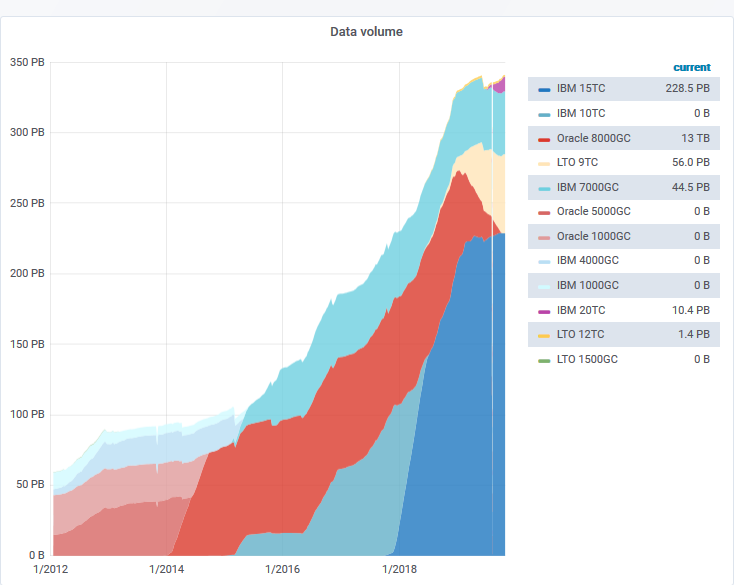
\includegraphics[keepaspectratio, height=1\textheight, width=1\textwidth]{../images/Tape_Stats_by_Density_History.png}
			\end{center}
		\end{column}
		\begin{column}{0.45\textwidth}
			\adjustbox{minipage=1.30\textwidth, scale=0.8}{{\Huge{}\textcolor{cern}{Latest development (I)}}
			  Repack
			  \begin{itemize}
			    \item Behind the scene operations for tape repair, free space reclaim, media migration...
			    \item Completion of repack enables production operations
			  \end{itemize}
			  Requests queueing
			  \begin{itemize}
			    \item Queueing was further optimized to reach \SI{250}{\hertz}
			  \end{itemize}
			}
		\end{column}
	\end{columns}
\end{frame}
\begin{frame}{Latest development (II)}
  Retrieve scheduling: Activities scheduling 
  \begin{itemize}
    \item Following discussions with ATLAS
    \item Intra-VO scheduling (other experiments unaffected)
    \item Prevents high latency for small request during big retrieve campaign
  \end{itemize}
  Retrieve scheduling: FIFO scheduling
  \begin{itemize}
    \item Avoids starving small mounts forever in high activity periods
    \item Optional switch between per-size or pre-age scheduling for retrieve (in development)
  \end{itemize}
\end{frame}

\subsection{Multiple database backends}
\begin{frame}{Tape file catalogue}
  \begin{itemize}
    \item 3 backends for production: Oracle, PostgreSQL, MySQL
    \begin{itemize}
      \item Oracle used for migration and current production
      \item Targeting future production on PostgreSQL (no schedule yet)
      \item MySQL support contributed by IHEP (Chinese Academy of Science). Many thanks to them!
    \end{itemize}
    \item All flavors validated (like all of CTA) in continuous integration tests
    \begin{itemize}
      \item See \textcolor{cern}{\href{https://indico.cern.ch/event/773049/contributions/3473307/}{``System testing CERN physics archival software using Docker and Kubernetes''}}
    \end{itemize}
  \end{itemize}
\end{frame}

\section{Migration from CASTOR to CTA}
\begin{frame}{Migration from CASTOR to CTA}
  \begin{itemize}
    \item Metadata-only migration: tape format unchanged
    \item Migration from a single CASTOR namespace to 5 EOSCTA instances
    \item Oracle to Oracle for CASTOR $\rightarrow$ CTA
    \item Injection tool for CASTOR $\rightarrow$ EOS
    \item Migration experiment by experiment
    \item Requires preparation and cleanup on CASTOR side
    \item Can be done as a read-only import (validated during ATLAS test)
    \item Typical time few hours
  \end{itemize}
\end{frame}

\section{Future functionality}
\begin{frame}{Future functionality}
  \begin{itemize}
    \item Provide fast positioning on LTO
    \begin{itemize}
      \item Software solution addressing lack of drive-provided recommended access order (RAO)
    \end{itemize}
    \item Pre-emptive scheduling
    \item Study of dataset collocation (PhD student)
    \item Various operations related features (drive dedication...)
  \end{itemize}
\end{frame}


\section{Conclusions}
\begin{frame}{Conclusions}
  \begin{itemize}
    \item EOSCTA core ready for production usage
    \item Promising tests validated the deployment model
    \item Delivered full tape performance on limited hardware
    \item Migrations of experiments at various stages, some requiring adaptation in the pipeline
    \item Focus in 2020 will be migration out of CASTOR for LHC experiments
  \end{itemize}

\end{frame}
\backcover
\end{document}